% This is the Latex template for my future homework write-ups
% A basic form of Latex command: '/command name[argu, argu]{argu*}' as below:
\documentclass[12pt, letterpaper]{article} % use 'tab' to complete 
% which means this document is an article with 12pt (font size) and letterpaper (paper type)


% ======================================================
% This is the preamble section for loading packages, a basic form looks like: 
% /usepackage{filename} the package name is the .sty file.  Let's load some 
% packages (Latex will complain if the .sty file is not in PWD):
% ======================================================
\usepackage{indentfirst} % indent the 1st line of the 1st paragraph, using \noindent to cancel
\usepackage{amsmath} % basic mathematic 
\usepackage{graphicx} % for using graphics
\usepackage{array} % for using arrays
\usepackage{lineno}   % for adding line numbers
\usepackage[authoryear]{natbib}   % for citing, more options see 'natbib'
\usepackage[notref,notcite]{showkeys} % easy to check the #name of each \ref
\usepackage{bm}  % Use the bold mode in math 
\usepackage{ulem} % added lines for our text, i.e., underline...
\usepackage{xcolor} % used for adding color to our text
\usepackage{listings} % used for displaying the highlight code

\usepackage{listings}
\usepackage{xcolor}

% ============================================================================
% These are basic settings for making title and content
% ============================================================================
% Now, we start the work by entering the document with:
\begin{document}  % always remember 'begin - end' pairs
% Basic settings for the title page
\title{\LaTeX: Phys 5391 Assignment - 5} % title name
\author{Yu Hong\\Space Physics Group} % double-slash for new line
\date{December 04, 2020}  % or the \today command to insert today's date.
% Now setting the format of the article
\maketitle % make a title based on  the info above
%\newpage % make a new page
%\tableofcontents % make a content page
%\newpage % make a new page
\linenumbers % turn on the line numbers.


% ============================================================================
% This Section is used for demonstrating some basic command of controlling paragraph and texts
% ============================================================================

\section{Minimal Substorm Model} % adding new section
% add  a new paragraph

The \textbf{minimal substorm model } is used here to examine substorms in 2003. This model considers the general state of the magnetospheric system and focuses on the evolution of the global dynamical state of the magnetotail during the substorm, which involves only three simple rules has been developed. This model is driven by the real solar wind power input, and can produces a probability distribution of times between substorm onsets that compares favourably with the observation. In this assignment, we first quantify \emph{the occurrences of substorms based on different parameter}, e.g., D (the period between substorms under constant solar wind driving), then analyze \emph{the general characteristics of substorms in different \textbf{seasons}, \textbf{UT time distribution} and \textbf{time interval} between two consecutive subtstorms}. Finally, with the corresponding Dst data, which as an indicator of geomagnetic storms, we checked the \emph{relationship between substorms and storms}. 


% ============================================================================
% This Section used for writing mathematics stuffs, the equation and table will be showing here
% ============================================================================
\section{Substorms Substorms Everywhere} % Start a new section for math
\subsection{Substorm occurrence with Parameters} % Start a subection for this part
At any given time, there exists an \textit{energy state E in the magnetotai} in the MSM can be written as follow:

% use the environment {equation} and label the equation as equ1
\begin{equation} 
  E = C - DP
  \label{eq:1}  
\end{equation} % end the environment {equation}

here, E is the magnetotail energy state at given time; D is the related substorm period parameter, generally D=2.69 hours as an standard input; P is the energy determined by solar wind conditions; C is a critical energy threshold, which we set as zero in our study. First, let's check parameter D:

% We'll see more of this syntax explained below (e.g., the !h).
\begin{table}[!h] % use the environment {table}
  \begin{center} % use the environment {environment}
  \begin{tabular}{|l|c|c|r|} % make a table with 4 colums: left, center, center, right
    \hline % Used to draw horizontal lines
    D (hours) & 2.6 & 2.69 &  2.9\\ % make a new line
    \hline % Used to draw horizontal lines
    \hline % Used to draw horizontal lines
    substorms & 1388 &1338 & 1251\\ % make a new line
    \hline % Used to draw horizontal lines
  \end{tabular} % end the environment {tabular}
  % Caption and label commands are key.
  \caption{The substorm occurrences changes with period parameter D} % add caption to this table
  \label{tab:tab1} % label the table, when quoting, \label and \ref appear in pairs
  \end{center} % end the environment {center}
\end{table} % end the environment {table}

In summary, the substorm occurrences increase with the decrease of period parameter D and decrease with the enhancement of D. This suggests that, the shorter the waiting time, the more likely it is to have a substorm. 

Next, let's examine the substorm occurrences change with P, we use three methods to get the initial energy P: 1. average of the day; 2. maximum of the day; and 3. the real value at 00UT of the day. The corresponding results are shown as follow:


% We'll see more of this syntax explained below (e.g., the !h).
\begin{table}[!h] % use the environment {table}
  \begin{center} % use the environment {environment}
  \begin{tabular}{|l|c|c|r|} % make a table with 4 colums: left, center, center, right
    \hline % Used to draw horizontal lines
    P (method) & ave & max &  real\\ % make a new line
    \hline % Used to draw horizontal lines
    \hline % Used to draw horizontal lines
    substorms & 1338 & 857 & 1447\\ % make a new line
    \hline % Used to draw horizontal lines
  \end{tabular} % end the environment {tabular}
  % Caption and label commands are key.
  \caption{The substorm occurrences changes with initial energy P} % add caption to this table
  \label{tab:tab2} % label the table, when quoting, \label and \ref appear in pairs
  \end{center} % end the environment {center}
\end{table} % end the environment {table}

In summary, the substorm occurrences increase with the decrease of initial energy P and decrease with the enhancement of P. This suggests that, the smaller the initial energy, the more likely it is to have a substorm. 

\subsection{Characteristics of Substorm Occurrence} % Start a subection for this part
First, let's check the occurrence of substorms in different seasons. Here, Equinox represents months of March, April, September and October; Summer represents months from May to August; Winter represents months of January, February, November and December. In general, Figure 1 suggests that the occurrences of substorm is not sensitive to season in 2003.

\begin{figure}[!t] % !b for bottom, t for top; ! for good position
\begin{center} % put the figure in the center 
  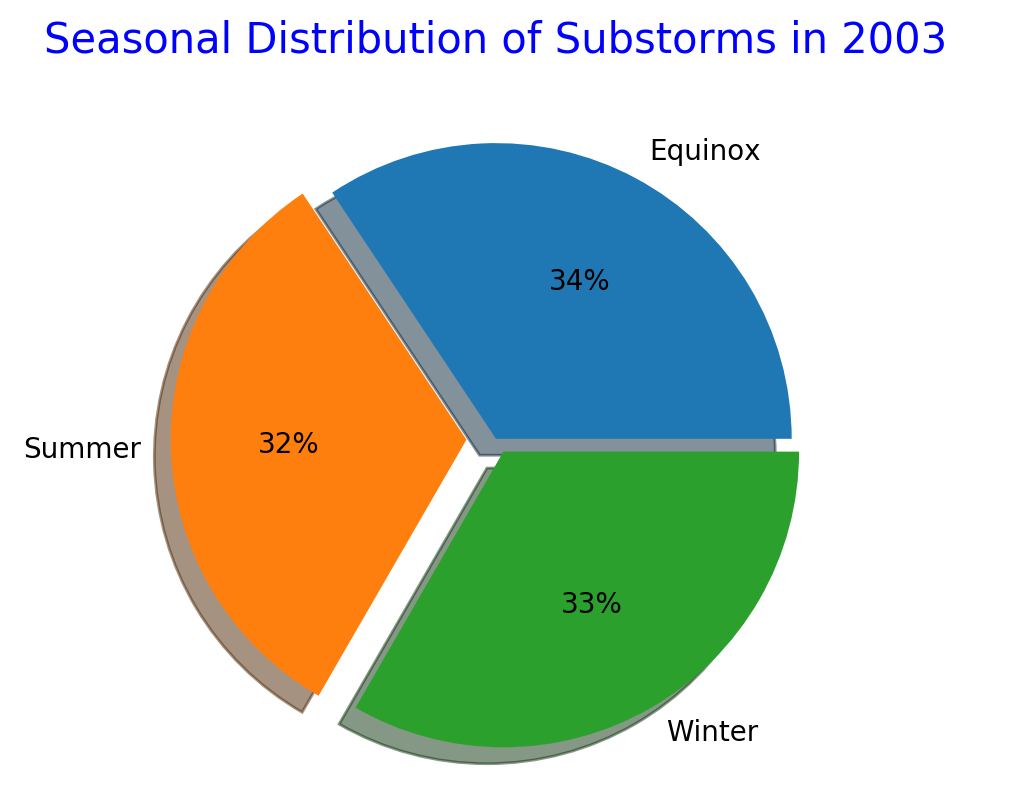
\includegraphics[width=8cm,height=6cm]{seasonal_distribution.png} % changing figure size and rotate: scale=1.2, angle=45
  \caption{Occurrence of substorms in different seasons} % This figure is in the same path as the code
  \label{fig:1} % label the figure with the unique name "rick"
\end{center} % end the environment {center}
\end{figure} % end the environment {figure}

Next, let's check the occurrence of substorms in different UT times. As shown in Figure 2, the left plot shows the UT times distributions of all the substorms in 2003, generally speaking, there is no significant difference between daytime and nighttime; The right figure shows the time interval between the two consecutive substorms, definitely, two consecutive substorms are more likely to occurred within 5 hours, while very few time intervals exceed 20 hours.

\begin{figure}[!t] % !b for bottom, t for top; ! for good position
\begin{center} % put the figure in the center 
  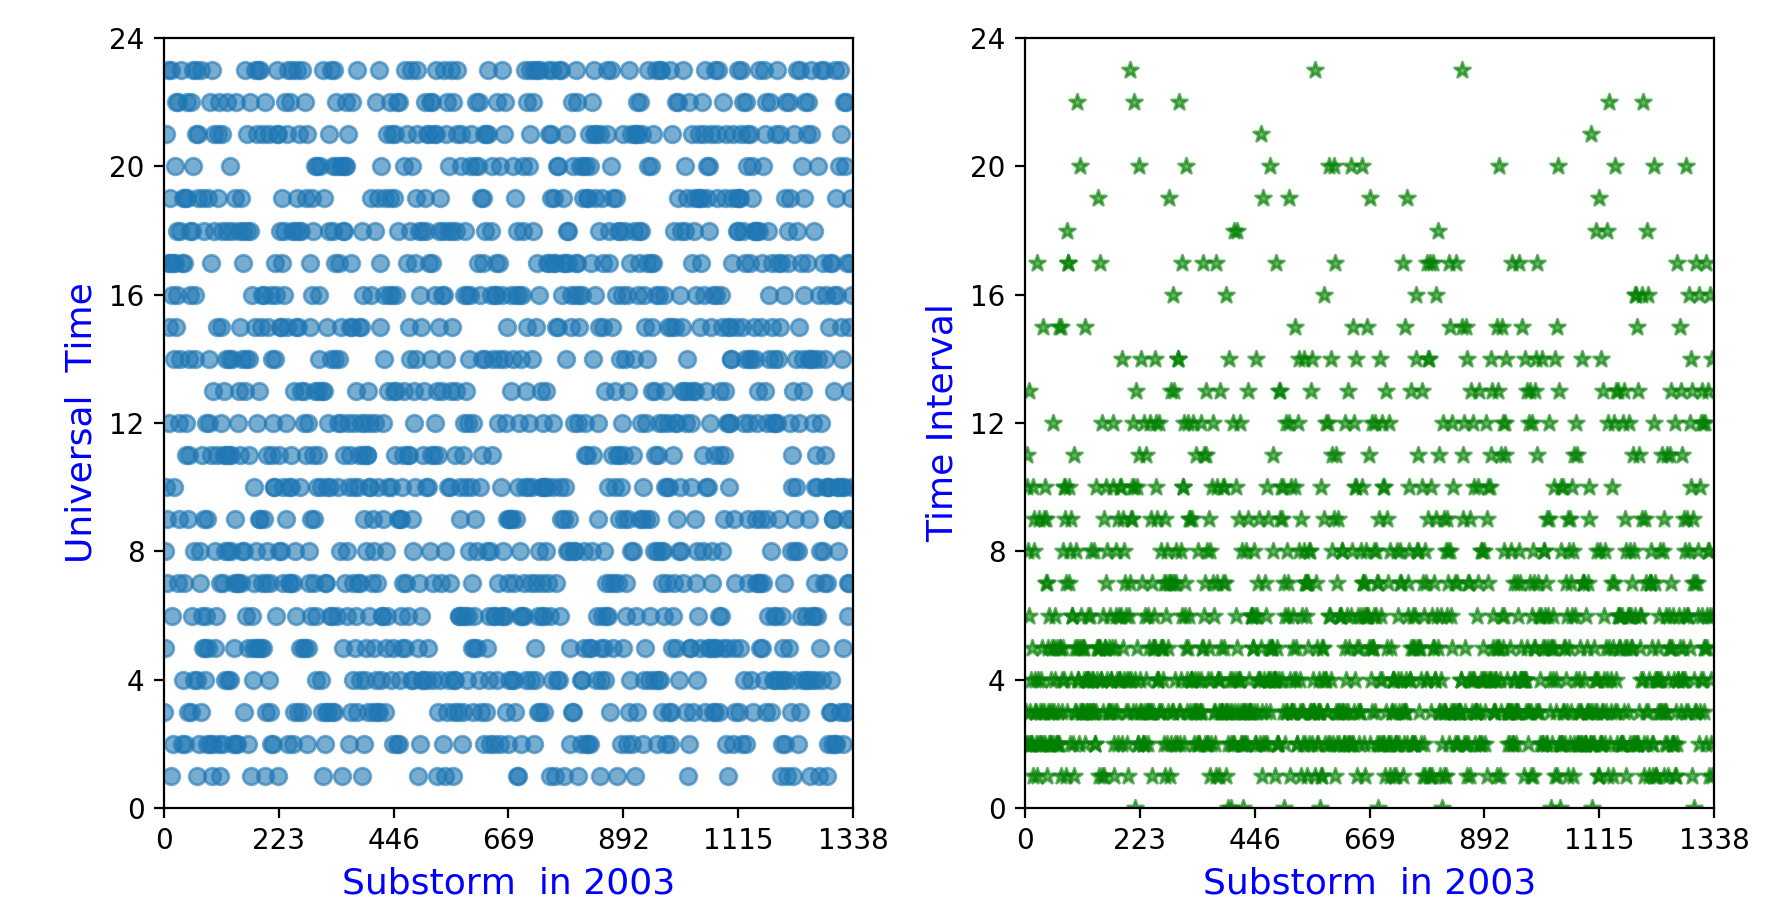
\includegraphics[width=8cm,height=6cm]{Time Interval.png} % changing figure size and rotate: scale=1.2, angle=45
  \caption{Occurrence of substorms in different UT times} % This figure is in the same path as the code
  \label{fig:2} % label the figure with the unique name "rick"
\end{center} % end the environment {center}
\end{figure} % end the environment {figure}


% ============================================================================
% This Section is used for demonstrating some other useful environments in Latex
% ============================================================================
\section{Substorms + Substorms = Storms ?} % Start a new section for other environments

Now, let's check the relationship between substorms and storms. In general, the model prediction of substorms are a bit crazy, there are more than 1,000 substorms happen in 2003. However, observations of storms show that the results are not so high frequency as substorms. For example, following figure 3 shows the geomagnetic storms happened in January of 2003, only one evident storm which occurred in 29th Jan was observed (~-60 nT). If we check the output data file of MSM in January, there are ~100 substorms provided. This means no very close connection between these two phenomena. 

\begin{figure}[!t] % !b for bottom, t for top; ! for good position
\begin{center} % put the figure in the center 
  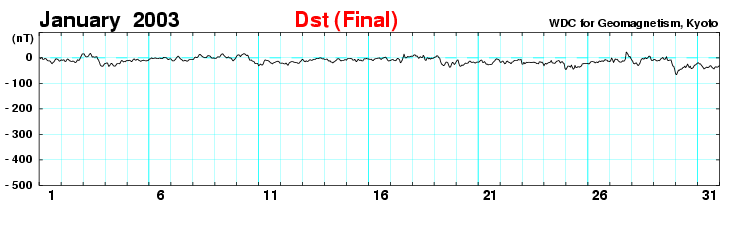
\includegraphics[width=15cm,height=6cm]{dst_200301.png} % changing figure size and rotate: scale=1.2, angle=45
  \caption{Occurrence of substorms in different UT times} % This figure is in the same path as the code
  \label{fig:3} % label the figure with the unique name "rick"
\end{center} % end the environment {center}
\end{figure} % end the environment {figure}



% ===================================================
% This Section is the demonstration of  how to Use Bibtex 
% ===================================================
% for the bibliography, these two lines are Very Useful.
\clearpage % make a new page 
\addcontentsline{toc}{section}{Bibliography} % make a section in the table of contents
% Using Bibtex, we just use these two lines to add the bib!
\bibliographystyle{plainnat} % plainnat is the standard plain format
\bibliography{assignment1} % assignment1 is the name of my bibtex file

% End the document environment.  This is the last line for coding
\end{document}










